\section*{Math 202a - HW2 - Dan Davison - \texttt{ddavison@berkeley.edu}}

Grade: 89 (100 pts possible)
Graded Anonymously: no
Comments:

5.2. You've got the right idea in the irrational case, but you haven't quite finished the argument. You need to
invoke Bolzano–Weierstrass or an equivalent result to extract a convergent (hence Cauchy) subsequence of the
orbit.

Ian Francis, Sep 21 at 8:57pm

4.2. Your argument that $F$ is continuous has a serious issue: the $F_n$ are uniformly Cauchy, and the
fundamental theorem of calculus *does* imply that the antiderivative of a Riemann integrable function is
continuous, but it does not follow that the antiderivative is differentiable (in fact, it is *not*
differentiable on the Cantor set), so you cannot conclude that the $F_n$ are Lipschitz.

Aidan Backus, Sep 23 at 8:09am

2. 10 3. 10 4. 8 5. 7

Ian Francis, Sep 25 at 4:42pm


On average, most students did quite well on Homework 2. Ian may have some comments about the "irrational rotation" problem, or possibly not; other than that, I think students struggled the most on problem 4, wherein one was given a mysterious function $F$, the Devil's staircase, that was somehow differentiable with zero derivative almost everywhere and yet surjective! Thus derivatives of functions which are not differentiable *everywhere* do not play nicely with measure theory. Here I think most of you had the idea of what to do, but resorted to horribly overcomplicated arguments, or worse, arguments that lacked enough detail to be complete.

For part 4a, wherein you had to show that the Devil's staircase was well-defined, I think it would've been helpful to think of the Cantor set as the set of infinite binary strings. If the nth bit in a binary string is 0, go left; otherwise go right. Then $F_n(x)$ is determined by the first n bits in x, and for every $\varepsilon > 0$ you can choose $x_1 < x < x_2$ and an n so large that $F_n(x_2) - \varepsilon \leq F_n(x_1) \leq F(x) \leq F_n(x_2)$. (Note that $F(x)$ in general is determined by all of the bits of x, which is why it is necessary to pass to $F_n$.) Then take $\varepsilon \to 0$. After 4a the problem is smooth sailing: apply the fundamental theorem of calculus, which says that $F$ is continuous (*and no more than continuous*).

Homework 3 was quite a bit tougher, owing to exercise 2.12 (no countable sigma-algebras). A lot of students didn't finish 2.18 (stochastic arithmetic) but those who did got most of the ideas, at least, right. By the way, since 2.18 was so long, we assigned triple credit for it this week.

One common approach to 2.12 involved choosing an arbitrary sequence of distinct measurable sets $A_n$ and mapping binary sequences $k_n$ into something like $\bigcup_n B_n$ where $B_n = A_n$ if $k_n = 1$ and $B_n = A_n^c$ else. A nice exercise would be to show that this does not work if the $A_n$ are, for example, a chain: $A_n \subseteq A_{n+1}$. The idea here isn't bad, but one needs to be very careful in how one chooses the $A_n$.

So it's tempting to consider the sets $A_\omega = \bigcap \{B: \omega \in B\}$, but one immediately runs into two problems: the $A_\omega$ may not be measurable, and of course the map $\omega \mapsto A_\omega$ is not injective if $\Omega = \mathbb Z$ and the measurable sets are generated by sets of the form $\{-n, n\}$ (why not?) By imposing an equivalence relation on $\Omega$ many of you overcame the latter problem. The former is more subtle: the problem asks you to show that the $\sigma$-algebra has cardinality at least that of $\mathbb R$, but many of you said that if this failed then the $\sigma$-algebra was in bijection with $\mathbb N$ (which implies that $A_\omega$ is measurable), and so fell victim to Cohen's forcing theorem: it is NOT true that every uncountable set has cardinality at least that of $\mathbb R$ unless one makes some very special hypotheses on the underlying logical system we are using!!

I wrote a lot more about my thoughts about 2.12, including a rather combinatorial proof that I cooked up, at this blog post: https://backus.home.blog/2020/09/28/boolean-algebras-and-probability/ -- really, the problem that it's so hard is that it has nothing to do with measure theory and everything to do with infinite combinatorics. I use the word "standard Borel space" a few times, but whenever I say that you can just think $\mathbb R$.

\begin{mdframed}
  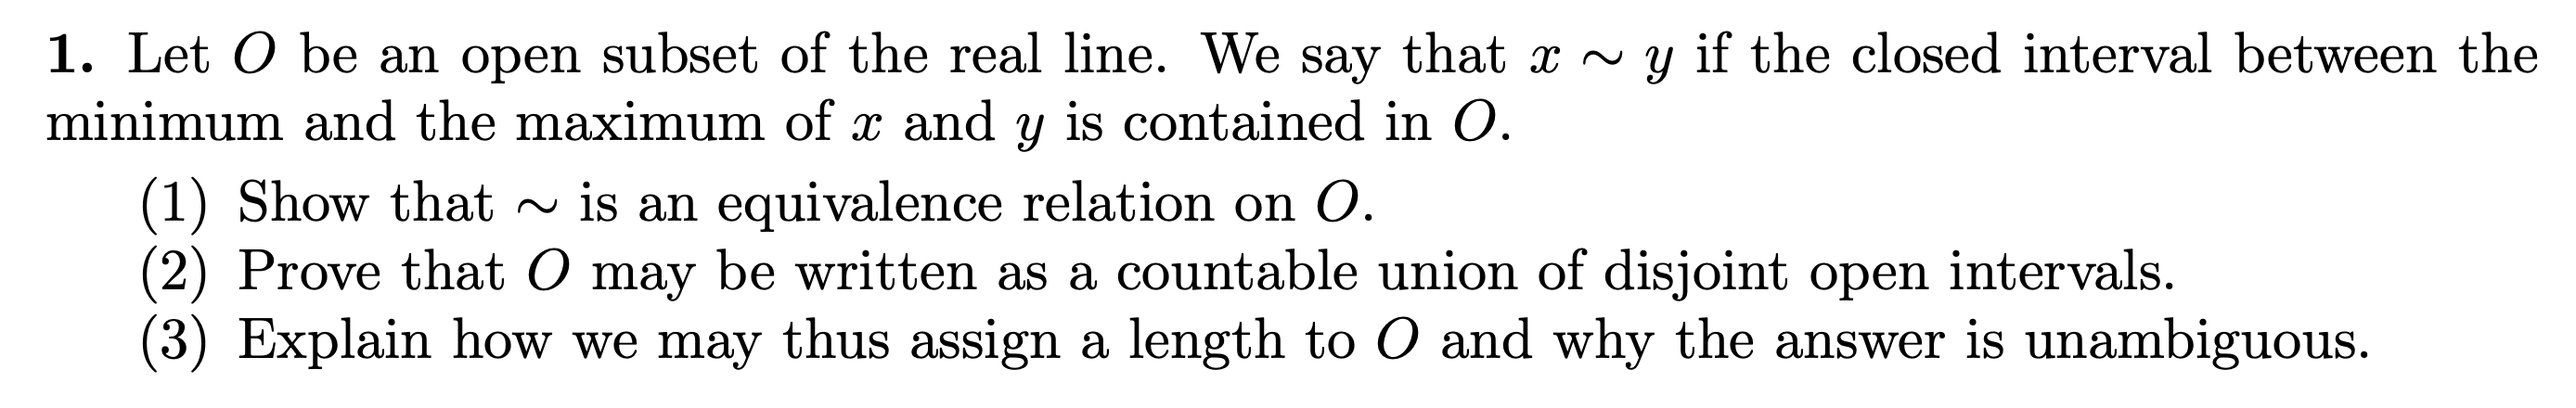
\includegraphics[width=400pt]{img/analysis--berkeley-202a-ebe4.png}
\end{mdframed}

\begin{intuition*}
  $O \subset \R$ is a countable union of disjoint open intervals.

  $x \sim y$ iff $x$ and $y$ are in the same interval.

  The length of $O$ should be the sum of the lengths of the intervals.
\end{intuition*}


\begin{enumerate}[label=(1.\arabic*)]
\item
  \begin{claim*}
    $\sim$ is an equivalence relation on $O$.
  \end{claim*}
  \begin{proof}
    \begin{enumerate}
    \item {\bf Reflexivity}\\
      $x \sim x$ since $[x, x] = \{x\} \subseteq O$.

    \item {\bf Symmetry}\\
      Let $x, y \in \R$ such that $x \sim y$. Then $[\min\{x, y\}, \max\{x, y\}] \subseteq O$.
      Therefore $[\min\{y, x\}, \max\{y, x\}] \subseteq O$. Therefore $y \sim x$.

    \item {\bf Transitivity}\\
      Let $x, y, z \in \R$ such that $x \sim y$ and $y \sim z$. Then $[\min\{x, y\}, \max\{x, y\}] \subseteq O$
      and $[\min\{y, z\}, \max\{y, z\}] \subseteq O$. Therefore $[\min\{x, y\}, \max\{y, z\}] \subseteq O$.
      Therefore $x \sim z$.
    \end{enumerate}
  \end{proof}

\item
  \begin{claim*}
    $O$ may be written as a countable union of disjoint open intervals.
  \end{claim*}

  \begin{proof}
    Let $\mc I = I_1, I_2, \ldots$ be the set of equivalence classes of $O$ under $\sim$.

    Since $\sim$ is an equivalence relation, the elements of $\mc I$ are disjoint and their union is equal
    to $O$.

    We now show that the elements of $\mc I$ are open sets. Let $I \in \mc I$ and suppose for a contradiction
    that $I$ is not open. Then there exists $x \in I$ such that no neighborhood of $x$ is contained within $I$.
    Let $x$ be such a point. Since $O$ is open, we may choose $\eps > 0$ such
    that $(x-\eps, x+\eps) \subseteq O$. Since $I$ is not open, for all $\eps' < \eps$, we have
    that $(x-\eps', x+\eps')$ contains a point outside $I$ in some other interval $J \in \mc I$
    where $J \neq I$. But this contradicts the disjointness of the partition $\mc I$. Therefore $I$ is open.

    Note that $I$ has at least two elements since $I$ is an equivalence class. It follows from transitivity of
    the equivalence relation that the elements of $\mc I$ are intervals.

    % Finally we show that the elements of $\mc I$ are intervals. Let $I \in \mc I$. Note that $I$ has at least
    % two elements since $I$ is an equivalence class. Suppose $I$ is bounded below and above. Then for
    % any $\epsilon > 0$ there exists $a \in I$ such that $a - \inf O < \epsilon$. Note that $[a, x] \subseteq I$
    % for all $x \in I$ where $a < x$. By a similar argument, $[x, b] \subseteq I$ for all $x \in I$
    % where $b = \sup I$ and $x < b$.  of the form $(I_a, I_b)$

    Finally we show that this is a countable union.

    Note that every rational number is in zero or one interval, but not more than one. Furthermore, every open
    interval contains at least one rational.

    Therefore there is a non-injective surjection from a subset of the rationals to the set of intervals.

    Therefore the cardinality of the set of intervals is not greater than the cardinality of the rationals.

    Therefore the set of intervals is countable.
  \end{proof}

\item
  \begin{proof}
    We may assign a length $\mu(O)$ to $O$ as follows:

    If $O = \emptyset$ then $\mu(O) := 0$.

    Otherwise, if $O$ is not bounded below, or if $O$ is not bounded above, then $\mu(O) := \infty$.

    Otherwise, if the series $\sum_i |I_i|$ diverges, then $\mu(O) := \infty$.

    Otherwise, $\mu(O) := \sum_i |I_i|$.

    Note that every term of the series is positive. In order for this definition to be unambiguous, the
    value $\mu(O)$ must not depend on the ordering of the series. This is true by the lemma below.
  \end{proof}

  \begin{lemma*}
    Let $\sum_i a_i$ be a series with $a_i > 0$ for all $i$. Then
    \begin{enumerate}
    \item If the series diverges for any ordering of the series, it diverges for all orderings.
    \item If the series converges for any ordering of the series, it converges to the same value for all
      orderings.
    \end{enumerate}
  \end{lemma*}
  \begin{proof}
    A sketch proof of the second statement is as follows: given any $\epsilon > 0$ we can identify a tail of
    the sequence whose sum is less than $\epsilon$. Thus the sum of the series is determined by the finite
    head. The sum of this finite head does not depend on its ordering, by commutativity of addition.
  \end{proof}
\end{enumerate}


\newpage
\begin{mdframed}
  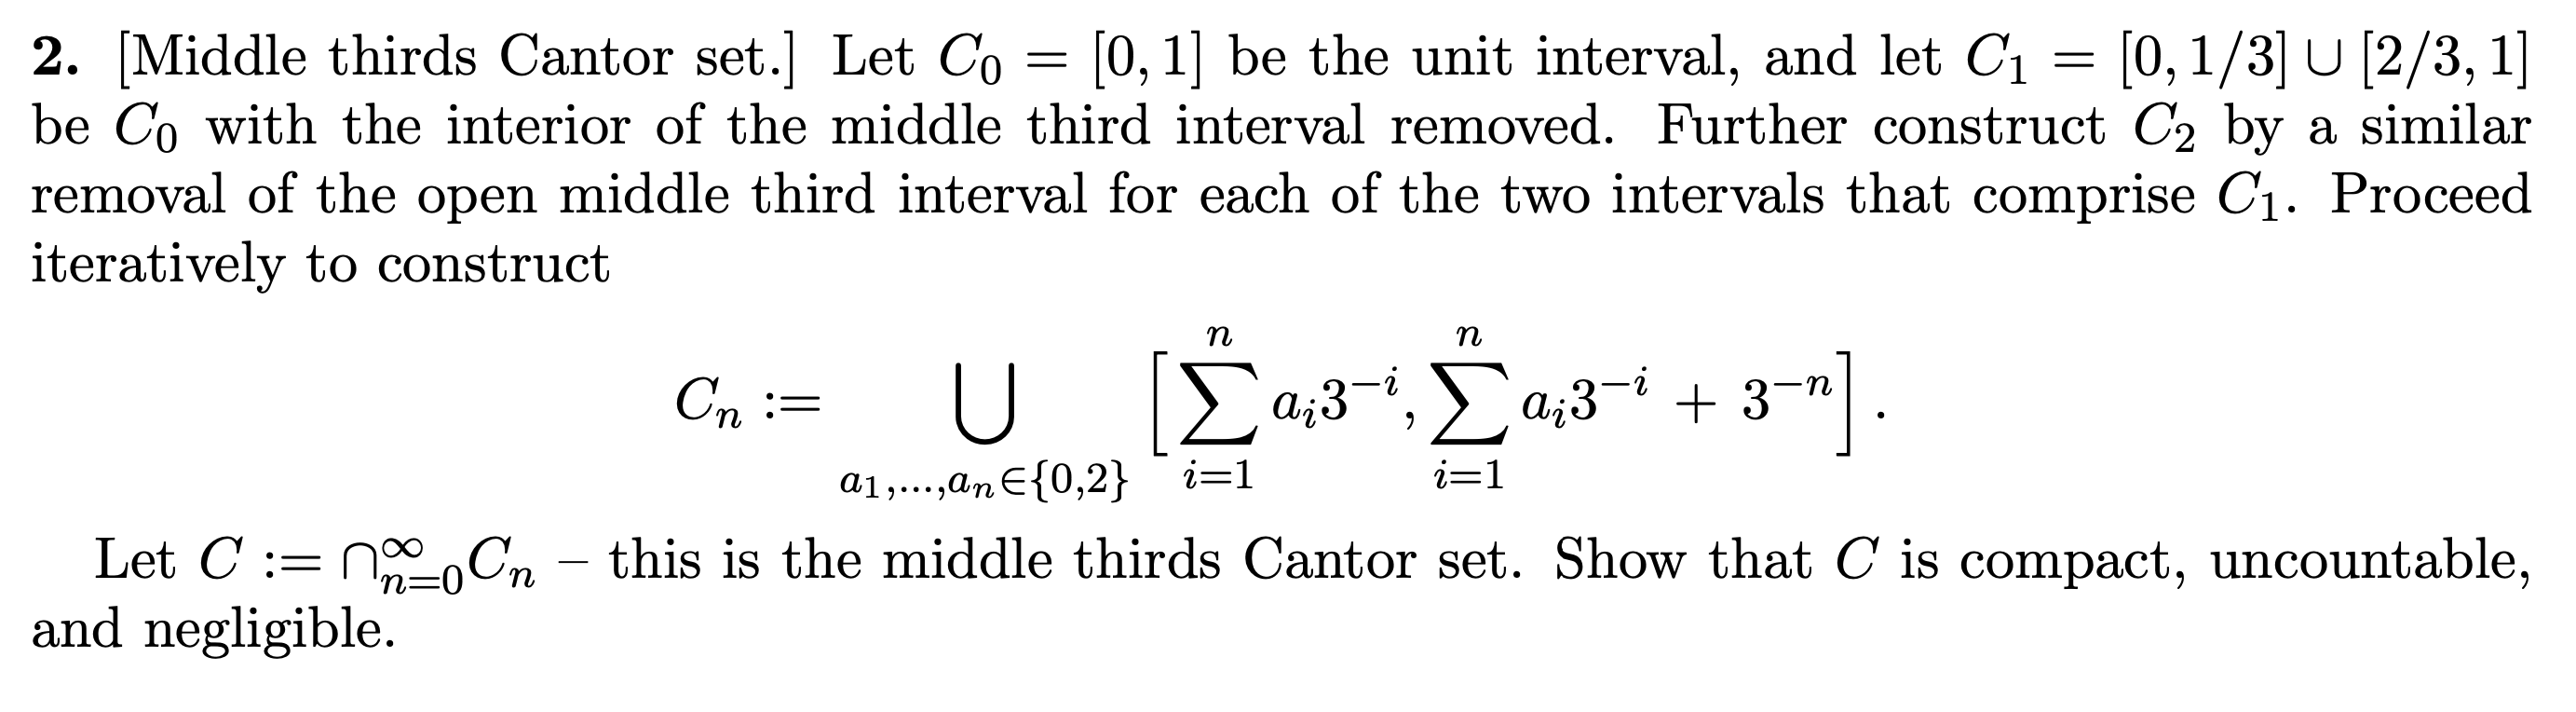
\includegraphics[width=400pt]{img/analysis--berkeley-202a-8d78.png}
\end{mdframed}

\begin{enumerate}[label=(2.\arabic*)]
\item
  \begin{claim*}
    $C$ is compact.
  \end{claim*}
  \begin{proof}
    Since $C \subset \R$ it suffices to show that $C$ is closed and bounded. Then it follows from the Heine-Borel
    theorem that $C$ is compact.

    $C$ is bounded below by $0$ and above by $1$, since it is constructed by removing points from $[0, 1]$.

    To show that $C$ is closed we may show that $C^c$ is open. Since $C = \bigcap_{n=0}^\infty C_n$, we
    have $C^c = \bigcup_{n=0}^\infty C_n^c$. Note that $C_n$ is a union of closed intervals; therefore $C_n^c$
    is a union of open intervals and therefore open (if an interval contains a neighborhood of each one of its
    points then the union of intervals also contains neighborhoods of those points); therefore $C^c$ is a union
    of open intervals and therefore open. Therefore $C$ is closed.
  \end{proof}

\item
  \begin{claim*}
    $C$ is uncountable.
  \end{claim*}

  \begin{proof}
    Note that $\om \in C$ if and only if the base 3 (ternary) expansion of $\om$ contains no $1$s.

    Consider the map $f:C \to [0, 1]$ defined by the following rule: $f(\om)$ is equal to the real number whose
    binary expansion is formed by substituting every $2$ with a $1$ in the ternary expansion of $\om$.

    This map is a bijection, therefore the cardinality of $C$ is equal to that of $[0, 1]$, therefore $C$ is
    uncountable.
  \end{proof}

\item \begin{claim*}
    $C$ is negligible.
  \end{claim*}

  \begin{proof}
    Fix an arbitrary $\epsilon > 0$. We will show that there exists a countable union of
    intervals $I_1, I_2, \ldots$ that cover $C$ and for which $\sum_k |I_k| < \epsilon$.

    Note that $C_n$ comprises $2^n$ disjoint intervals each of length $3^{-n}$. Therefore the total length
    of $C_n$ is $|C_n| = \big(\frac{2}{3}\big)^n$ and we see that $|C_n| < \epsilon$ for
    all $n > \Big\lceil\frac{\log\eps}{\log 2/3} \Big\rceil$. Since $C \subset C_n$ for all $n$, we see
    that $|C| < \eps$. We can write $C$ as $C = \bigcup_{k=1}^\infty I_k$, and so we can construct an efficient
    cover for $C$ as follows: for $k \in \{1, 2, \ldots\}$ place an interval of length $2^{-k}\eps$ over $I_k$.
    The total length of the cover is $\eps\sum_{k=1}^\infty 2^{-k} = \eps$.

%    \red{TODO} Tie this up by giving explicit coordinates for the intervals in the covering.
  \end{proof}

\end{enumerate}

\newpage
\begin{mdframed}
  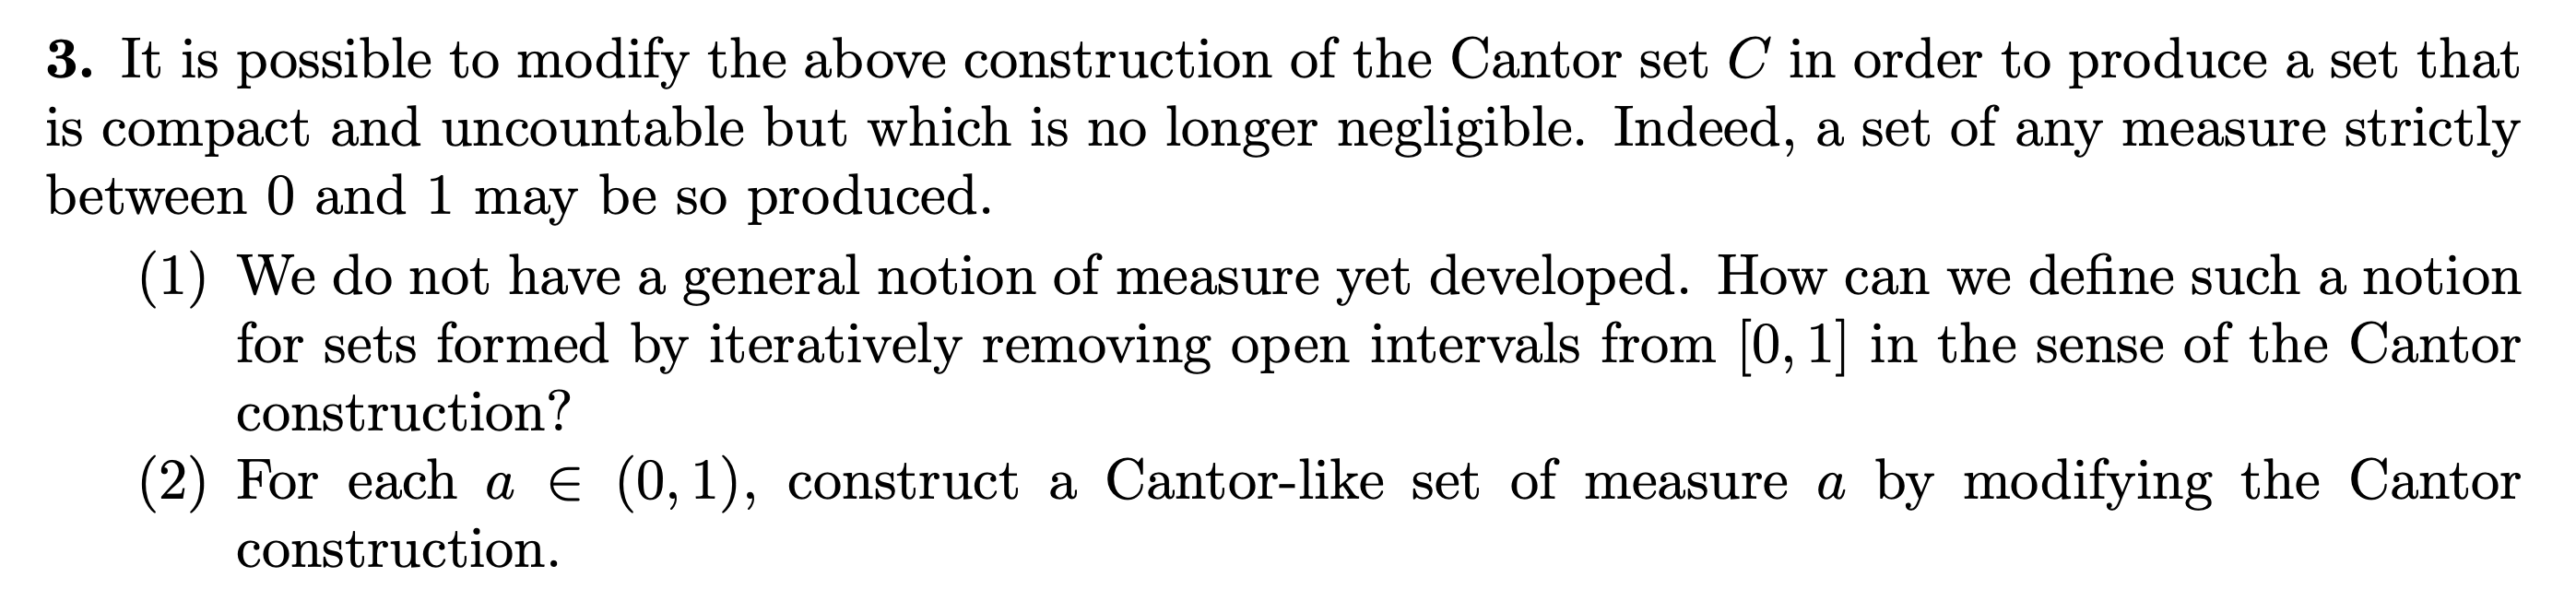
\includegraphics[width=400pt]{img/analysis--berkeley-202a-6b7a.png}
\end{mdframed}

\begin{enumerate}[label=(3.\arabic*)]

\item
  \begin{definition*}
    Let $X$ be a set formed by iteratively removing open intervals from $[0, 1]$. Let $I_1, I_2, \ldots$ be the
    open intervals that were removed in the formation of $X$. Note that these are disjoint, since a point can
    not be removed more than once. Define the measure of $X$ to be $1 - \sum_k |I_k|$.
  \end{definition*}

\item
  \begin{definition*}[Cantor set of measure $a$]
    Let $a \in (0, 1)$. The Cantor set of measure $a$ is formed as follows:

    Instead of removing $1/3$ at each iteration, we will remove a smaller fraction.

    Note that $\sum_{n=1}^\infty \frac{1 - a}{2^n} = 1 - a$. So we will design an algorithm that
    removes $\frac{1-a}{2^n}$ at each iteration, for $n=1, 2, \ldots$. Note that at the start of iteration $n$
    we have $n$ intervals. Therefore, in order to remove a length of $\frac{1-a}{2^n}$ we will remove the
    middle $\frac{1-a}{n2^n}$ from each interval.

    \red{TODO} It's not true that there are $n$ intervals at the start of iteration $n$. There are $2^n$ intervals. So
    we have to remove $\frac{1-a}{2^{2n}}$ from each interval.
  \end{definition*}
\end{enumerate}



\newpage
\begin{mdframed}
  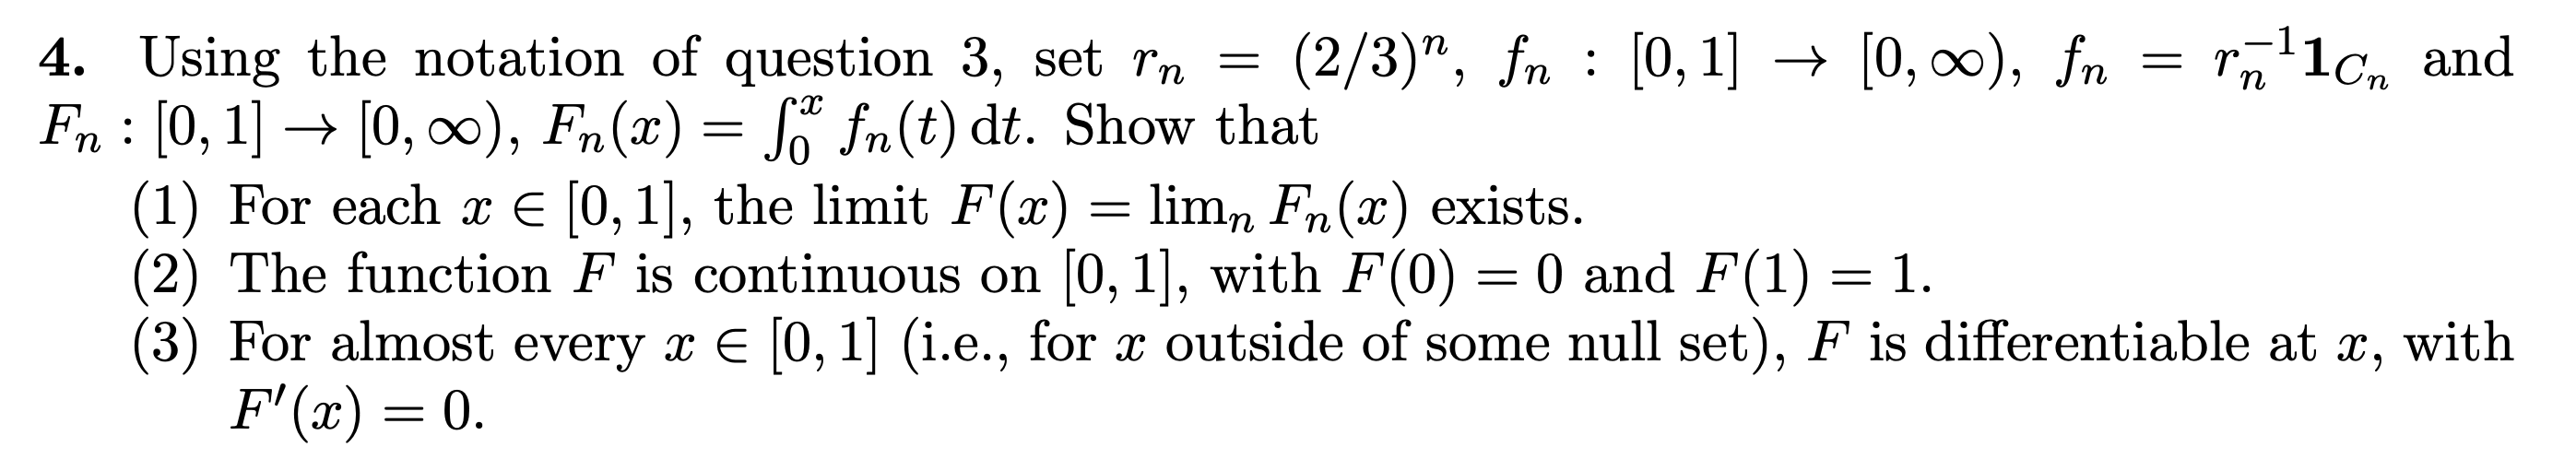
\includegraphics[width=400pt]{img/analysis--berkeley-202a-8ce8.png}
\end{mdframed}

\begin{lemma}\label{lemma-4-1}
  $F_n(1) = 1$ for all $n$.
\end{lemma}

\begin{proof}
  For all $n$ we have that $C_n$ is a union of $2^n$ intervals, each of length $1/3^n$, therefore the total
  length is decreasing: $|C_n| = (2/3)^n$. The function $f_n$ has the value $(3/2)^n$ on each interval in $C_n$
  and zero elsewhere. Therefore $F_n(1) = \(\frac{3}{2}\)^n\(\frac{2}{3}\)^n = 1$ for all $n$.
\end{proof}

\begin{lemma}\label{lemma-4-2}
  Let $x \in C^c$. There exists $m$ such that $F_{n+1}(x) = F_n(x)$ for all $n > m$.
\end{lemma}
\begin{proof}
  Let $x \in C^c$. Then there exists $m$ such that for all $n > m$ we have $x \in C_n^c$. Let $m$ be such a
  value and fix an arbitrary $n > m$. We write $C_n$ as a union of $2^n$ closed
  intervals, $C_n = \bigcup_{i=1}^{2^n} [a_i, b_i]$, and let $k = |\{i \in \{1, \ldots, 2^n\} ~:~ b_i < x\}|$
  be the number of these intervals whose right endpoints are less than $x$. We have
  \begin{align*}
    F_n(x) = k\Big(\frac{3}{2}\Big)^n\Big(\frac{1}{3}\Big)^n = \frac{k}{2^n}.
  \end{align*}
  At the next generation, there are $2k$ of these intervals whose right endpoints are less than $x$, and we
  have
  \begin{align*}
    F_{n+1}(x) = 2k\Big(\frac{3}{2}\Big)^{n+1}\Big(\frac{1}{3}\Big)^{n+1} = \frac{k}{2^n}.
  \end{align*}
  Therefore $F_{n+1}(x) = F_n(x)$ for all $n > m$.
\end{proof}


\begin{lemma}\label{lemma-4-3}
  Let $[a, b] \subset C$. Then $\int_a^b \big|f_{n+1}(x) - f_n(x)\big| \dx = \frac{1}{3}\frac{1}{2^{n-1}}$.
\end{lemma}

\begin{proof}
  Let $[a, b] \subset C$. For $x$ in the left or right thirds (closed) of this interval we have
  \begin{align*}
    f_{n+1}(x) - f_n(x)
    = \Big(\frac{3}{2}\Big)^{n+1} - \Big(\frac{3}{2}\Big)^{n}
    = \frac{1}{2}\Big(\frac{3}{2}\Big)^n,
  \end{align*}
  and for $x$ in the middle third (open) of this interval we have
  \begin{align*}
    f_{n+1}(x) - f_n(x)
    = -\Big(\frac{3}{2}\Big)^{n}.
  \end{align*}
  Since the interval has length $(1/3)^n$ we have
  \begin{align*}
    \int_a^b \big|f_{n+1}(x) - f_n(x)\big| \dx
    &=  \frac{2}{3}\Big(\frac{1}{3}\Big)^n\frac{1}{2}\Big(\frac{3}{2}\Big)^n
      + \frac{1}{3}\Big(\frac{1}{3}\Big)^n\Big(\frac{3}{2}\Big)^n \\
      % &= \Big(\frac{1}{3}\Big)^n\Big(\frac{3}{2}\Big)^n\Big(\frac{2}{3}\frac{1}{2} + \frac{1}{3}\Big) \\
    &= 2\Big(\frac{1}{3}\Big)^{n+1}\Big(\frac{3}{2}\Big)^n\\
    &= \frac{1}{3}\frac{1}{2^{n-1}}.
  \end{align*}
\end{proof}


\begin{enumerate}[label=(4.\arabic*)]

\item
  \begin{claim*}
    For each $x \in [0, 1]$ the limit $F(x) = \lim_{n\to\infty} F_n(x)$ exists.
  \end{claim*}

  \begin{proof}
    We will study the difference $|F_{n+1}(x) - F_n(x)|$ and show that this decreases with $n$ in a way that
    implies that the sequence $F_0(x), F_1(x), \ldots$ is Cauchy for all $x \in [0, 1]$.

    First consider $x \in C^c$. Then from lemma \ref{lemma-4-2} we have that $F_{n+1}(x) - F_{n}(x) = 0$ for
    sufficiently large $n$ and so the sequence is obviously Cauchy at a point $x \in C^c$.

    Next let $x \in C$ and let $[a, b] \subset C$ be the closed interval containing $x$. Then
    \begin{align*}
      F_{n+1}(x) - F_n(x)
      &= \Big(\int_0^a f_{n+1}(t) \dt + \int_a^x f_{n+1}(t) \dt\Big)
        - \Big(\int_0^a f_{n}(t) \dt   + \int_a^x f_{n}(t) \dt\Big) \\
      &= F_{n+1}(a) - F_{n}(a)
        + \Big(\int_a^x f_{n+1}(t) \dt - \int_a^x f_{n}(t) \dt\Big).
    \end{align*}
    Now, from lemma \ref{lemma-4-2} we have that $F_{n+1}(x) - F_{n}(x) = 0$ for sufficiently large $n$,
    where $x \in C^c$. But this result also holds for $x$ an endpoint of a closed interval in $C$, since such
    an endpoint is arbitrarily close to a point of $C^c$. Thus we have $F_{n+1}(a) - F_{n}(a) = 0$ and, using
    lemma \ref{lemma-4-3},
    \begin{align*}
      \Big|F_{n+1}(x) - F_n(x)\Big|
      &=    \Big|\int_a^x f_{n+1}(t) \dt - f_{n}(t) \dt\Big| \\
      &\leq \int_a^x \big|f_{n+1}(t) \dt - f_{n}(t)\big| \dt \\
      &\leq \int_a^b \big|f_{n+1}(t) \dt - f_{n}(t)\big| \dt \\
      &=    \frac{1}{3}\frac{1}{2^{n-1}} \\
      &<    \frac{1}{2^n}.
    \end{align*}
    In order to show that $F_0(x), F_1(x), \ldots$ is Cauchy, fix $0 < \eps < 1$, let $m \in \N$ be such
    that $\sum_{k=1}^m \frac{1}{2^k} \geq 1 - \eps$, and let $i, j > m$. Then
    \begin{align*}
      \Big|F_i(x) - F_j(x)\Big| \leq \sum_{k=m+1}^\infty \frac{1}{2^k} < \eps.
    \end{align*}
    Therefore the sequence $F_0(x), F_1(x), \ldots$ is Cauchy at a point $x \in C$.

    Since the sequence $F_0(x), F_1(x), \ldots$ is Cauchy for all $x \in [0, 1]$, the
    limit $F(x) = \lim_{n\to\infty} F_n(x)$ exists for all $x \in [0, 1]$.

    Furthermore, the same $m$ works for all $x$, i.e. the sequence is uniformly Cauchy.
  \end{proof}

\item
  \begin{claim*}
    $F$ is continuous on $[0, 1]$ with $F(0) = 0$ and $F(1) = 1$.
  \end{claim*}

  \begin{proof}
    For continuity of $F$ it suffices to prove that the $F_n$ are continuous, since in part (4.1) we proved
    that they are uniformly Cauchy and hence converge uniformly to $F$. Continuity of $F$ then follows from the
    uniform limit theorem.

    Informally, the $F_n$ are piecewise affine and thus obviously continuous. To prove this, note that from
    the fundamental theorem of calculus we have that $F'_n = f_n$. Therefore $|F'_n|$ is bounded above
    by $(3/2)^n$, hence $F_n$ is Lipschitz continuous and therefore continuous.

    Finally, we have
    \begin{align*}
      F(0) &= \lim_{n\to\infty} \int_0^0 f_n(0) \dt = 0,
    \end{align*}
    and, from lemma \ref{lemma-4-1} we have
    \begin{align*}
      F(1)
      &= \lim_{n\to\infty} \int_0^1 f_n(t) \dt \\
      &= \lim_{n\to\infty} 1 \\
      &= 1.
    \end{align*}
  \end{proof}


\item
  \begin{proof}
    For every point $x \in C^c$, $F$ is constant within a neighborhood of $x$. Since we showed in question 2
    that $C$ is a null set (i.e. negligible), this implies that for $x$ outside a null set (``almost
    every $x$​'') $F$ is differentiable with $F'(x) = 0$.
  \end{proof}
\end{enumerate}


\newpage
\begin{mdframed}
  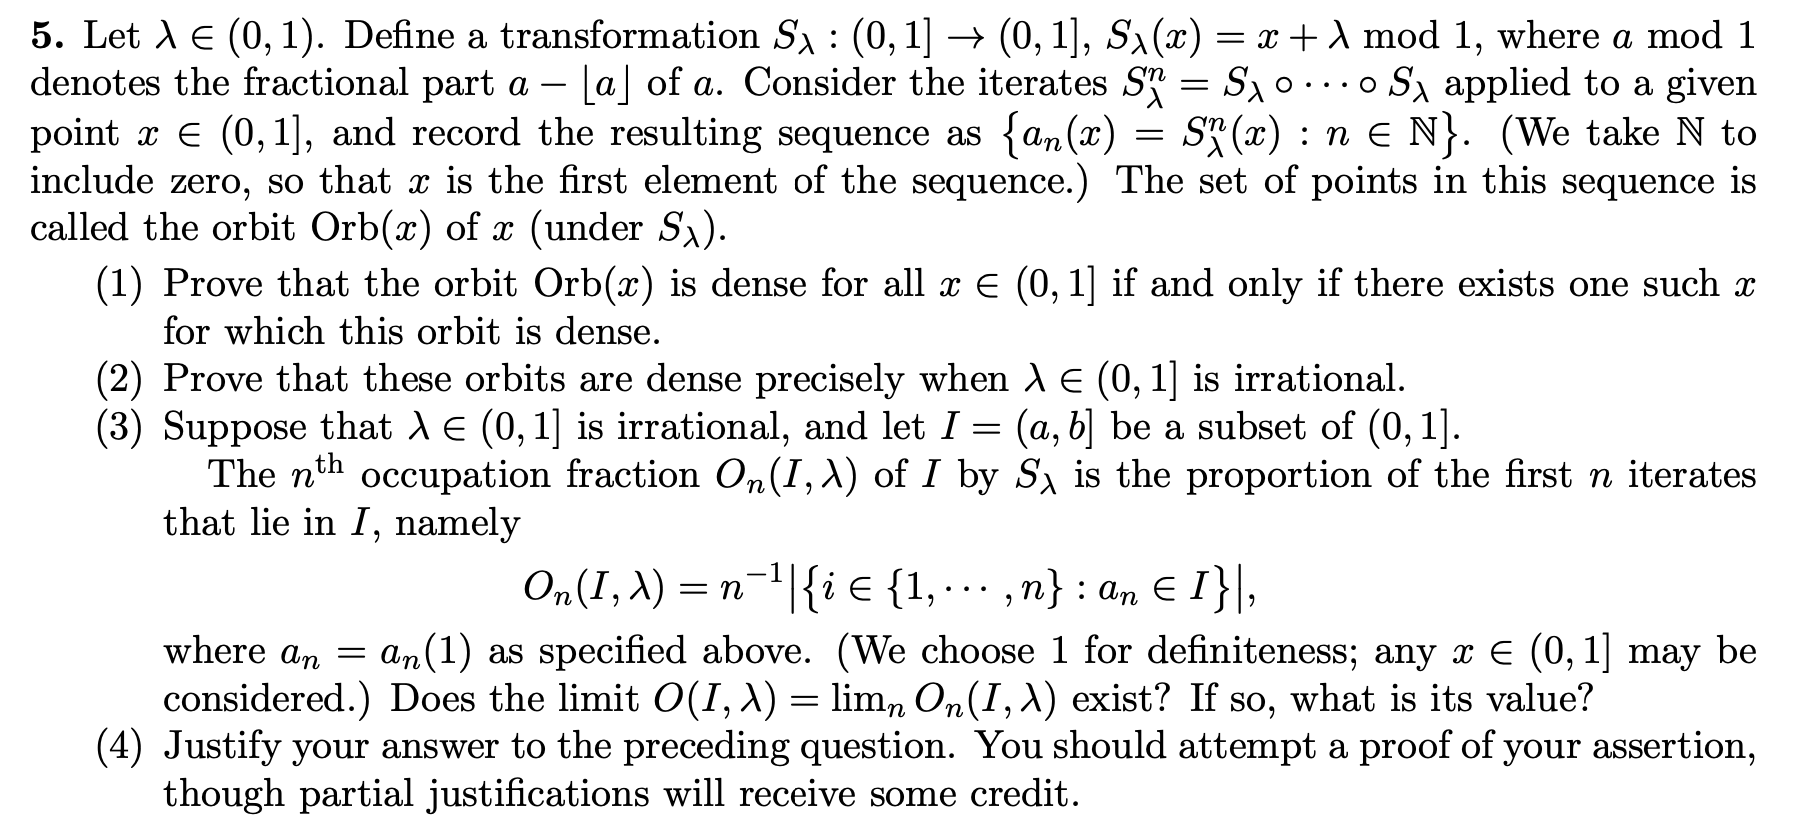
\includegraphics[width=400pt]{img/analysis--berkeley-202a-hw-8c2b.png}
\end{mdframed}

\begin{enumerate}[label=(5.\arabic*)]

\item
  \begin{claim*}
    The orbit $S_{\lambda}(x)$ is dense for all $x \in (0, 1]$ iff there exists an $x$ for which it is dense.
  \end{claim*}
  \begin{proof}
    Let $x$ be such that $S_\lambda(x)$ is dense. Let $y \neq x$. Since the orbit of $x$ is dense, the sequence
    starting at $x$ will visit a point $y'$ arbitrarily close to $y$. The set of points in the tail of the
    sequence, after visiting $y'$, is the orbit of $y'$. Since the orbit of $x$ is dense, the set of points in
    any tail is also dense, hence $\orb(y')$ is dense.

    But $y'$ differs from $y$ by an arbitrarily small epsilon. Since the transformation is additive, the $i$-th
    element in the sequence starting at $y$ differs from the corresponding element in the sequence starting
    at $y'$ by this same $\eps$. It follows that $\orb(y)$ is dense also.
  \end{proof}

\item
% \begin{lemma}\label{lemma-5-1}
%   \begin{align*}
%     S^n_\lambda(x)
%     &= x + S^n_\lambda(1) \mod 1 \\
%     &= x + n\lambda \mod 1
%   \end{align*}
% \end{lemma}
  \begin{claim*}
    The orbits are dense iff $\lambda \in (0, 1]$ is irrational.
  \end{claim*}
  \begin{proof}
    Let $j, k \in \N$ and let $\lambda = \frac{j}{k}$ be a rational number in reduced form.

    Note that $S^n_\lambda(x) = x + n\lambda \mod 1$. Therefore
    \begin{align*}
      S^k_\lambda(x)
      &= x + k\frac{j}{k} \mod 1 \\
      &= x + 1 \mod 1 \\
      &= x.
    \end{align*}
    Therefore if $\lambda$ is rational, the sequence returns to its starting point after finitely many
    iterations. Therefore $\orb(x)$ under $S_\lambda$ is a finite set, therefore it is not dense in $(0, 1]$.

    Now suppose $\lambda$ is irrational. Then
    \begin{align*}
      S^k_\lambda(x) = x + k\lambda \mod 1.
    \end{align*}
    Since $k\lambda = i$ has no solutions for irrational $\lambda$ and integers $i, k$, we see that the
    sequence never returns to its starting point.
  \end{proof}


\item
  \begin{definition*}
    The $n$-th occupation fraction of $I$ by $S_\lambda$ is
    \begin{align*}
      O_n(I, \lambda) = \frac{1}{n}\Big|\Big\{i \in \{1, \ldots, n\} ~:~ a_n \in I\Big\}\Big|.
    \end{align*}
  \end{definition*}
  \begin{claim*}
    The occupation fraction has a limiting value $\lim_{n\to\infty}O_n(I, \lambda) = b - a$.
  \end{claim*}
\item

  \begin{proof}[Proof sketch]
    Focus on the $j$-th digit in the binary expansion of $a_n$, and consider the orbit of that digit alone.
    That's a sequence of $0$s and $1$s that we may interpret as a real number in $[0, 1]$. The claimed result
    would be proved if we can prove the following:

    \begin{enumerate}
    \item The real number corresponding to the sequence visited by the $j$-th digit is normal, for all $j$.
    \item The sequence for digit $j$ becomes (in an appropriate sense) uncorrelated with the sequence for
      digit $k \neq j$.
    \end{enumerate}

    Those two results together would imply that each digit is visiting $0$ and $1$ with equal frequency,
    independently of other digits, and therefore that $a_n$ itself has no tendency to occupy any particular
    dyadic interval more than any other dyadic interval, from which the claimed result follows.

    In order to prove those results, I would investigate the following direction:
    \begin{enumerate}
    \item Note that $\lambda$ is irrational, therefore has a non-repeating binary expansion.

    \item Study the behavior of the binary expansion of $a_n$ under repeated addition of $\lambda$, i.e. with carrying and the mod 1 operation.
    \end{enumerate}
  \end{proof}

\begin{mdframed}
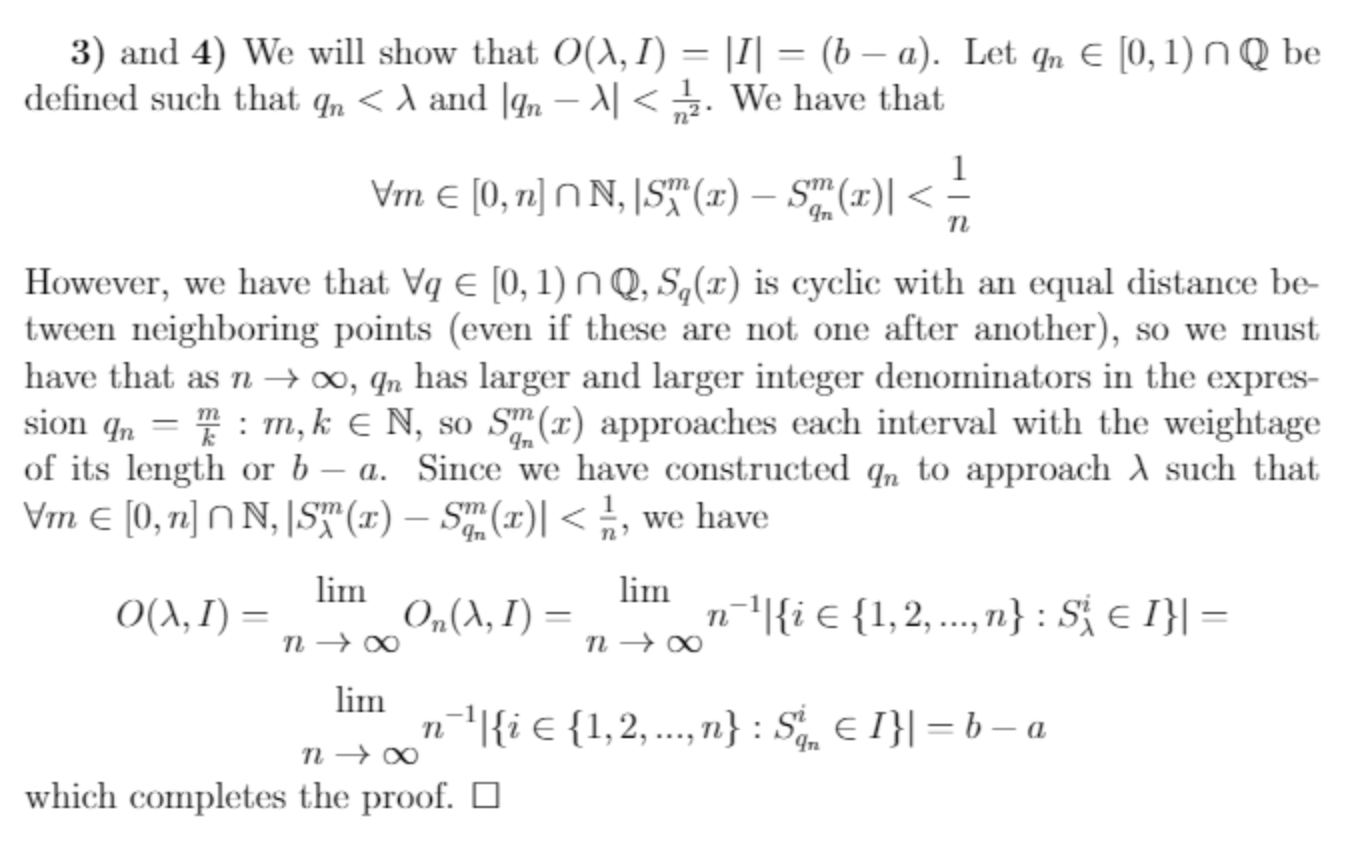
\includegraphics[width=400pt]{img/analysis--berkeley-202a-hw02-9a70.png}
\end{mdframed}

\end{enumerate}
